\chapter{Introduction}
\label{label:chapIntro}

\section{The Standard Model}
A physics model is a description of a system using physics and mathematical concepts and language.
Standard Model (SM) is a physics model that summarizes what is currently known about the subatomic world. The SM is composed of two gauge symmetry theories: the Glashow-Salam-Weinberg Model (GSW)~\cite{Glashow, Salam, Weinberg} describing electroweak interactions; the Quantum Chromodynamics 
(QCD)~\cite{QCD} describing the strong interactions. 
In SM, there are 
two types of fundamental particles, fermions and bosons. Fermions are the building block of matter,
and bosons are the intermediate particles of the four fundamental interactions of SM, i.e., strong, weak, electromagnetic, and
gravitational force. 
In this chapter, we briefly introduce the components of the SM and the related theories to this thesis. 
%A detailed elaboration about the SM could be found in books like Griffiths~\cite{particlebook1}. 


\subsection{Fundamental particles}

Fermions are defined as particles with half integer spin (intrinsic angular momentum), like leptons, quarks, proton, etc, while bosons are particles with integer spin, like the photon and the Higgs boson.
The fundamental particles of SM are shown in Figure~\ref{fig:SMParticles}. 

\begin{figure}[!htbp]
\centering
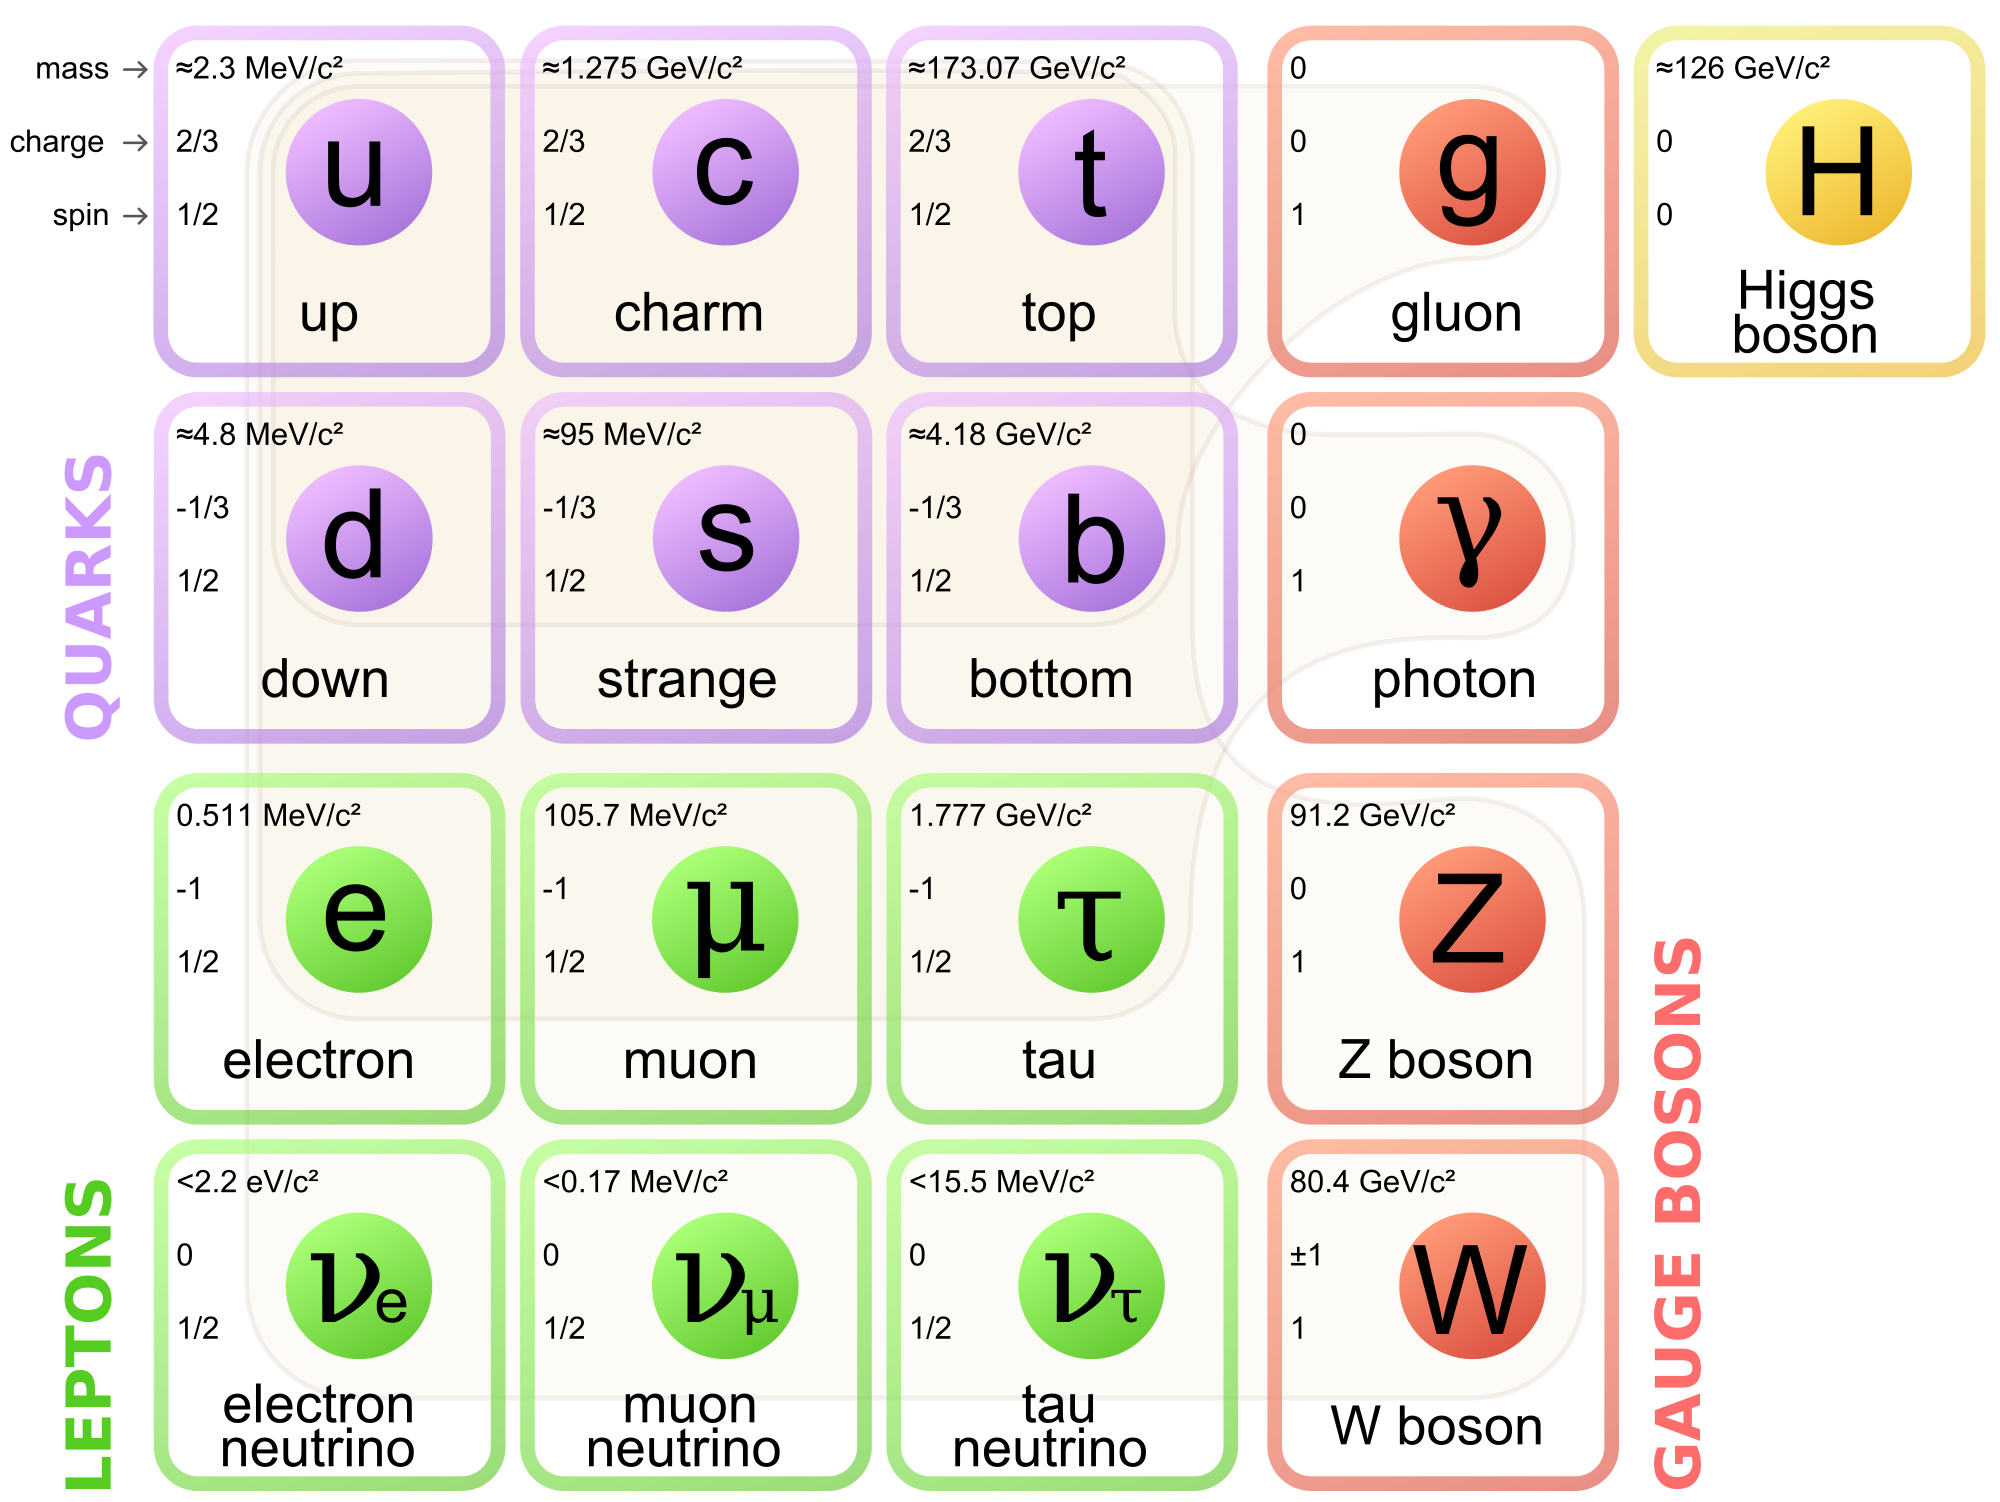
\includegraphics[width=.7\textwidth]{figures/Standard_Model_particles.png}
\caption{Standard model of elementary particles: 
the 12 fundamental fermions and 5 fundamental bosons.~\cite{particleImage}}
\label{fig:SMParticles}
\end{figure}  


{\bf Quarks}

In SM, there are six flavors of quarks: up (u), down (d), strange (s), charm (c), top (t), and bottom (b).  
Quarks carry properties like flavor, color, spin, charge, mass, etc. All quarks have spin $\frac{1}{2}$ in SM and they belong to one of the three generations: u and d quarks belong to the first generation; s and c quarks are the second generation quarks; t and b quarks 
make up the third generation. %The generation of quarks is mostly categorized by their coupling strength with each other in 
%the weak interactions and also their discovery time.  
The color is a property of particle. In Quantum Chromodynamics, color is conserved in strong interactions. 
There are normally 3 types of color: red, blue, green. A particle is colorless if it carries a net color 
charge of zero. 
  
%An anti-quark will carry the opposite charge and color compared with the quark, but the
%same flavor and mass.  

{\bf Leptons}

Leptons are fundamental particles, which are also fermions. 
As shown in Figure~\ref{fig:SMParticles}, there are three generation of leptons: electron (e) and electron neutrino ($\nu_e$) are the first generation; 
muon ($\mu$) and muon neutrino ($\nu_\mu$) are the second generation; 
tau ($\tau$) and tau neutrino ($\nu_\tau$) are the third generation.  Leptons 
have electronic charge,  but do not 
carry color charges. Thus they are involved in the electroweak interactions, but not the
strong interactions. 

{\bf Bosons}

Every interaction has its mediator: the photon ($\gamma$) for electromagnetic force,  W and Z boson for weak force, gluon ($g$) for strong force and 
graviton (not found yet) for gravity. Higgs boson (H), although not a mediator, 
accounts for the mass of other fundamental particles, which will be elaborated in the following section. 
The W, Z, $\gamma$ and $g$ bosons having spin 1, are called vector boson. H boson has spin 0, which is called a scaler boson. 
There are two W bosons, distinguished by their electron charges,  ${\rm W^+}$ and ${\rm W^-}$. 




%\subsection{Weak interactions of quarks}

%The charged weak interaction of quarks doesn't obey the "generation-conservation laws" of 
%leptonic weak interactions, which means W boson could decay to u, d quarks, while W 
%could also decay to u, s quarks.  

%{\bf CKM matrix}

\section{Fundamental interactions}

In SM, there are four fundamental forces : strong, electromagnetic,  weak and 
gravitational force, as shown in Table~\ref{table:fourForces}. The ``Strength'' column 
in Table~\ref{table:fourForces} is not the real strength of the force, 
but a value to show the relative strength of these forces. 

Since gravity is so small compared to other three forces, it is mostly not considered in 
the process of particle physics. 
The strong force is described by the Quantum Chromodynamics. And the electromagnetic force and 
weak force are unified into electroweak interaction, described by the
Glashow-Weinberg-Salam (GSW) model. 
The theory of particular interest to this thesis 
is the Quantum Chromodynamics (QCD), which will be introduced in the following section.  

\iffalse
\begin{table}[!htbp]
\begin{tabular}{cccc}
Force & Strength & Theory & Mediator \\
\hline 
Strong  & 10 &  Quantum Chromodynamics  & Gluon \\
Electromagnetic & $10^{-2}$ & Quantum Electrodynamics & Photon \\
Weak & $10^{-13}$ & GSW model & W and Z \\
Gravitational & $10^{-42}$ & not defined & Graviton \\
\hline 
\end{tabular}
\caption{Summary of the four fundamental forces in Standard Model~\cite{particlebook1}.}
\label{table:fourForces}
\end{table} 
\fi

\begin{table}[!htbp]
\center
\begin{tabular}{cccc}
Force & Strength & Mediator \\
\hline 
Strong  & 10 &   Gluon \\
Electromagnetic & $10^{-2}$ &  Photon \\
Weak & $10^{-13}$ & W and Z \\
Gravitational & $10^{-42}$  & Graviton \\
\hline 
\end{tabular}
\caption{Summary of the four fundamental forces in Standard Model~\cite{particlebook1}.}
\label{table:fourForces}
\end{table}


%Here in this section, we will briefly introduce the Quantum Electrodynamics (QED),  

\subsection{Quantum Electrodynamics (QED)}

QED is the theory describing the electromagnetic interaction: the 
interaction between electric charged particles via the exchange of photons. 
The primitive process in QED, in the form of Feynman diagram, is shown in 
Figure~\ref{fig:primitiveQED}. An electron comes in, and radiates a photon, then goes out. 
%This process is the building block of QED. 
By connecting couple of these primitive processes together, we can get complex process like the one in
Figure~\ref{fig:gluonradiation}. In Figure~\ref{fig:gluonradiation}, the electron and positron annihilate into a
photon, which further decays to a pair of quarks, and then one of the two quarks radiates a gluon. 
The photon in Figure~\ref{fig:gluonradiation} is a virtual particle. Virtual particles are not
observable, which are called ``off-shell" particles. While real particles, in Figure~\ref{fig:gluonradiation}, 
are the incoming electron and positron, and outgoing quarks and gluons, which can be observed and
are ``on-shell". 
 
\begin{figure}[!htbp]
\centering
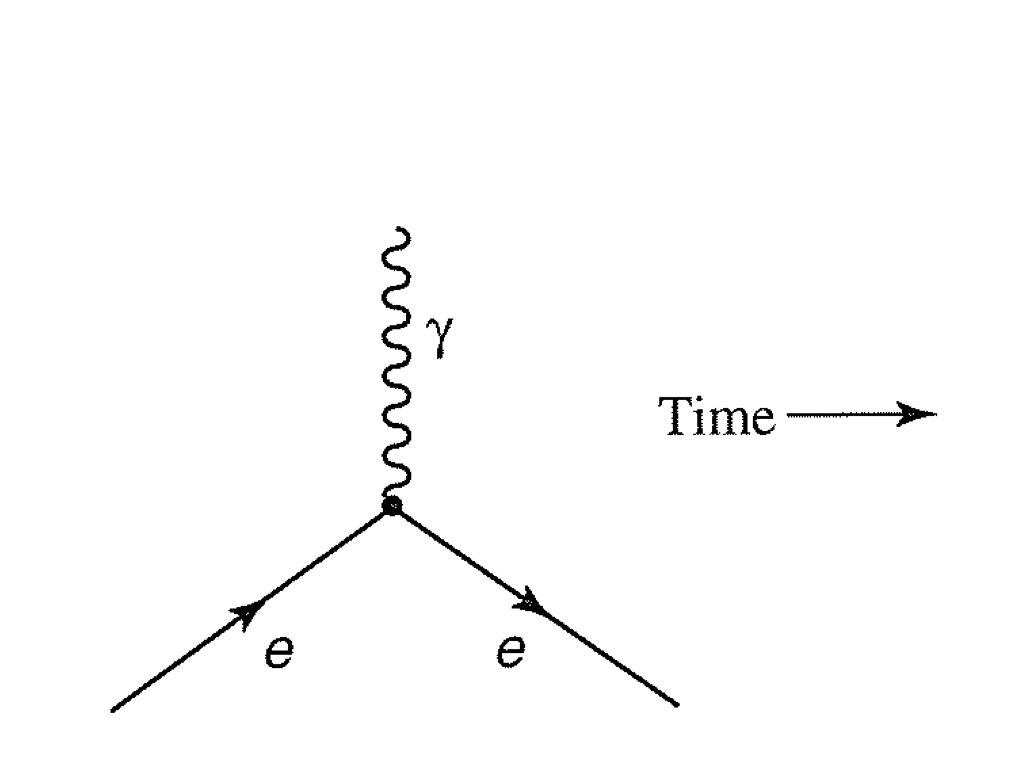
\includegraphics[width=.7\textwidth]{figures/primitiveQED.png}
\caption{The primitive QED process in SM. }
\label{fig:primitiveQED}
\end{figure} 

 
\begin{figure}[!htbp]
\centering
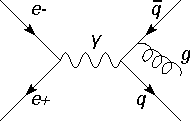
\includegraphics[width=.7\textwidth]{figures/Radiate_gluon.png}
\caption{Feynman diagram for electron annihilation.}
\label{fig:gluonradiation}
\end{figure} 


 
  
%The basic ``naive" process in QED, as shown in Figure~\ref{fig:basicFeyman}, is that
%an electron comes in, then radiates a photon and goes out. 
%It could 
%never happen standalone, because this againsts energy and momentum conservation. 
%However,  all other processes in QED could be built by this ``naive" process.  For example, 
%the BaBa scattering and Moller scattering, as shown in Figure~\ref{fig:baba} and ~\ref{fig:moller}. 


%\begin{equation}

%\end{equation}

 
%\subsection{}

%\subsection{W, Z and Higgs}


\subsection{Quantum Chromodynamics (QCD) and jets}

QCD is a theory describing the strong force and the involved fundamental particles. 
As we see from Table~\ref{table:fourForces}, strong force is the strongest force of the four. 
However, unlike the long range electromagnetic force, 
the strong force could only affect ${\rm {\approx} 10^{-15}~m}$ (1~fm), which is about the radius of 
a nucleus. 

Color is one of the unique properties of QCD. The color of QCD is an analogy to the charge of QED. There are three types of colors charges: red,
blue, green. Each quark carry one kind of color.
So, for example, there are 
three types of top quarks in QCD:  the blue top quark, the green top quark, and the red top quark.
This is the same for all the other five flavors of quarks.  
Anti-quark carries one kind of anti-color. 
Gluons is the boson intermediating the strong force, just like the
photon is the mediator of the electromagnetic force.
Gluons has a color and an anti-color. 
When two quarks interact with each other, 
they interact through a gluon by exchanging colors.
For example, as shown in Figure~\ref{fig:color_rb}, one red quark comes in, radiates a gluon with color red and anti-blue, 
and a blue quark goes out. In terms of the color SU(3) symmetry, there are 8 gluons in QCD, as
shown in Equation~\ref{eq:8colors}.

\begin{figure}[htb]
\centering
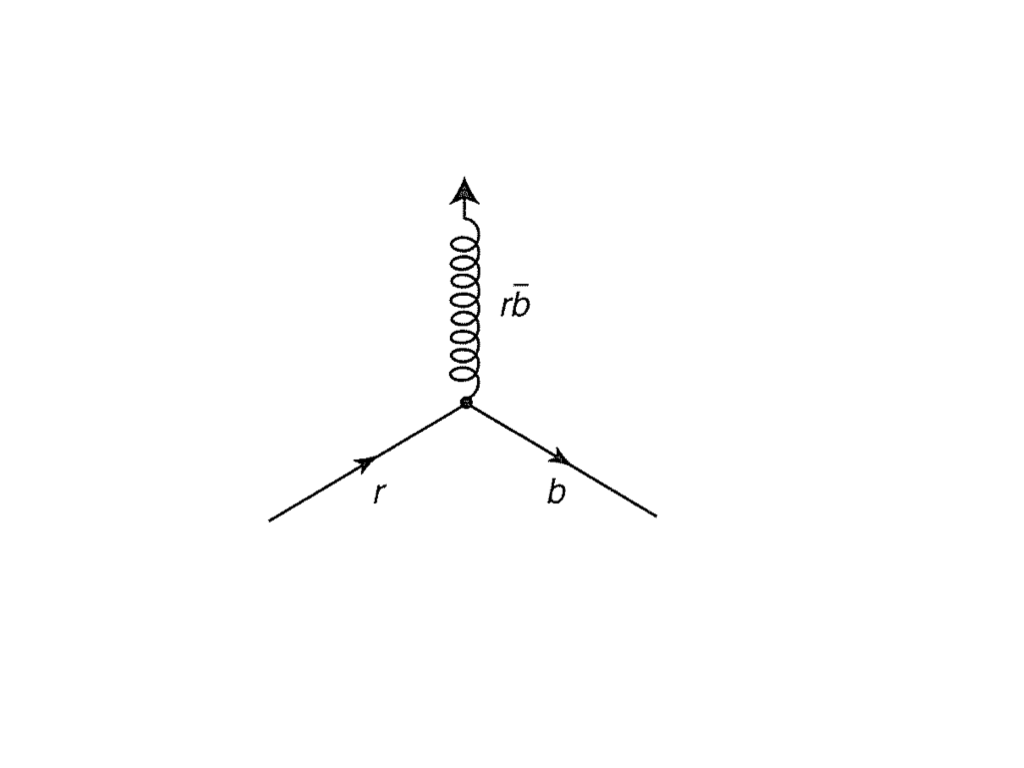
\includegraphics[width=.7\textwidth]{figures/rbcolor.png}
\caption{The illustration of quark-gluon interaction~\cite{particlebook1}.}
\label{fig:color_rb}
\end{figure}  

\begin{equation}
\begin{split}
(r\bar{b} + b\bar{r})/\sqrt{2}  \quad \quad \quad -i(r\bar{g}-g\bar{r})/\sqrt{2} \\
-i(r\bar{b}-b\bar{r})/\sqrt{2}   \quad \quad  \quad  (b\bar{g} + g\bar{b})/\sqrt{2} \\
(r\bar{r} - b\bar{b})/\sqrt{2}   \quad \quad  \quad  -i(b\bar{g} - g\bar{b})/\sqrt{2} \\
(r\bar{g} + g\bar{r})/\sqrt{2}   \quad \quad   \quad (r\bar{r} + b\bar{b} -2g\bar{g})/\sqrt{6} \\
\end{split}
\label{eq:8colors}
\end{equation}


Unlike charged particles, colored particle could not be free. What we see in experiments and daily life is 
color-singlet. So we can never observe a single quark or a single gluon 
in an experiment. 
What we observe is the ``hadronization" products of quarks and gluons, which are
called ``jets" and introduced in the following text. The existence of quarks and gluons is proved by indirect experiments via jets. 
Here we introduce the essential components of QCD. 
%The details about hodronization and jets are
%elaborated in the following text.  
%However, we can prove their existence by some other indirect measurements. 
%{\color{red} Here I might want to cite some experiment}

{\bf The coupling constant}

The coupling constant is a scaler quantity describing the strength of an interaction. 
Here in QCD, the coupling constant $\alpha_{s}$ is :
\begin{equation}
\alpha_{s}(|q^2|) = \frac{2\pi}{(11n-2f)ln(|q^2|/\Lambda^2)}   \quad (|q^2| \gg \Lambda^2)
\label{equation:coupling}
\end{equation}
where  $|q|^2$ is the squared energy-momentum 4-vector of the mediator gluon, $n$ is the number of colors (3, in SM), 
$f$ is the number of flavors (3, in SM), and $\Lambda$ is a parameter determined from 
experimental data, which is in the range of $100 {\sim} 500$~MeV. 

Notice that $\alpha_{s}$ is not a constant. It is a function of $|q|^2$. Because of this, it is also 
named the ``running coupling constant".  The experimental measurements are shown 
in Figure~\ref{figs:coupling}.

\begin{figure}[htb]
\centering
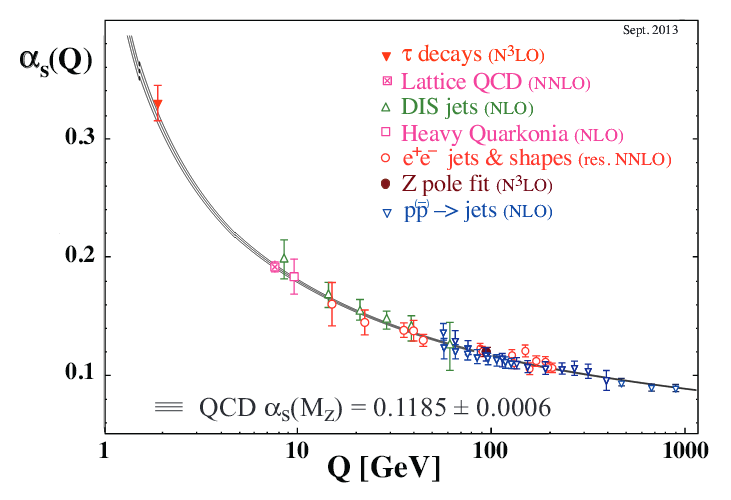
\includegraphics[width=.7\textwidth]{figures/alphasrunning.png}
\caption{The running coupling constant of QCD. NLO is short for the next leading order.
NNLO is short for next-next-leading order.}
\label{figs:coupling}
\end{figure}  

 
{\bf Asymptotic freedom}

As we see from Equation~\ref{equation:coupling}, 
when $|q|^2$ increases, $\alpha_{s}$ decreases. 
At  large $|q|^2$, corresponding to
short distances (${\leq}1~fm$),  the strong force 
is so weak that quarks inside of proton travel freely.  At very high energies, 
it is also possible to form quark-gluon plasma, since their interactions are so weak. 
This is called the asymptotic freedom. 

{\bf QCD confinement}


QCD confinement means that the force between quarks will hugely increase when they are separated. 
So one has to exert a lot energy to try to separate a quark from other quarks. And this energy will
become large enough for the mediator gluon to decay into a new quark pair. 
As illustrated in Figure~\ref{fig:color_field},  when the two charm quarks are pulled apart, the 
strong force between them increases, and the mediating gluon will have 
a large amount of energy. Before the $c\bar{c}$ quarks are further separated, the gluon  
creates a pair of $d\bar{d}$ quarks. This process continues,  and eventually the particle formed by 
$c\bar{c}$ quarks will become 
two particles formed by $c\bar{d}$ and $\bar{c}d$ quarks.
The gluon could create any pair of quarks, 
as long as its energy is large enough. Here we use $d\bar{d}$ quark pair as an illustration. 
Also $d\bar{d}$ quark pair requires relatively low energy to create, compared to other quark anti-quark pairs. 

\begin{figure}[htb]
\centering
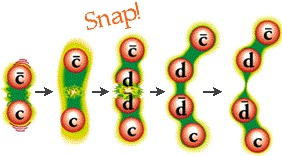
\includegraphics[width=.7\textwidth]{figures/color_field.jpg}
\caption{The illustration of QCD confinement~\cite{web:qcd_confinement}.}
\label{fig:color_field}
\end{figure}  



{\bf Jet formation}

When quarks and gluons are created in a high energy collision, they will
move away from the collision position freely for a brief moment. And then,
because of QCD confinement, when the quarks are separated by a distance
${\geq} 1~fm$, new quark pairs are created from the virtual gluons exchanged by 
the interaction between the initial quarks, as shown in Figure~\ref{fig:hadronization}. 
This process stops when the gluons or quarks don't have enough kinetic energy to create new
quark-aniquark pairs. The quarks or gluons initially created by the the energetic collision,
enentually become hadrons; this process is called hadronization. The stream of particles
created by the hadronization of a single quark or gluon is called a jet, as shown in 
Figure~\ref{fig:hadronization} and~\ref{fig:jet_formation}. 


\begin{figure}[!htbp]
\centering
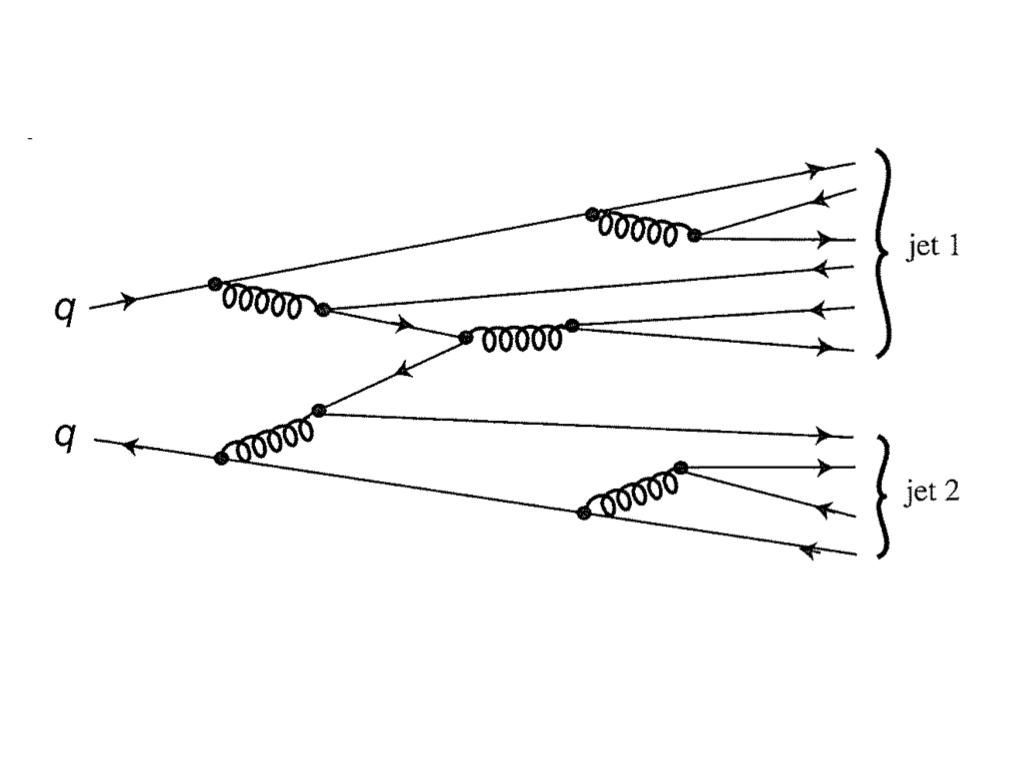
\includegraphics[width=.7\textwidth]{figures/jets.png}
\caption{The hadronization process~\cite{particlebook1}.}
\label{fig:hadronization}
\end{figure}  

\begin{figure}[!htbp]
\centering
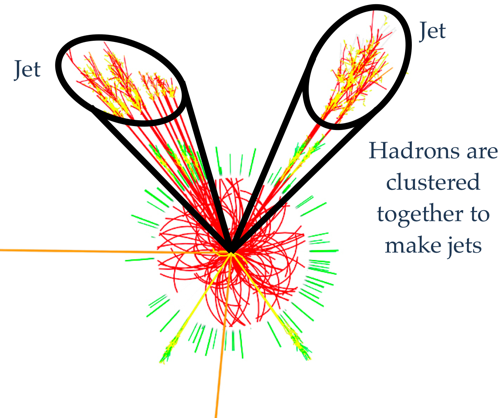
\includegraphics[width=.7\textwidth]{figures/clustering.png}
\caption{A sketch of jets formation in a high energy collision. Hadrons are clustered
together to make jets.}
\label{fig:jet_formation}
\end{figure}  

%\subsection{Charged weak interaction of quarks: CKM matrix}


\subsection{The SM Higgs mechanism}

The SM Higgs boson is a scaler boson, with spin 0. In SM, Higgs has a non-zero vacuum expectation
value (VEV), as shown in Figure~\ref{fig:Higgs}, while all other particles have zero VEVs. 
As shown in Figure~\ref{fig:Higgs}, the Higgs particle with the non-zero VEV is tending to slide down to the bottom of the potential. While the Higgs particle is on top of the potential, a rotation of the whole system in space-time dimensions, does not change its symmetry. However, when the Higgs particle is sliding off the potential to the bottom, as shown in Figure~\ref{fig:Higgs}, the rotation symmetry is broken. This is called the spontaneous symmetry breaking.  
The Higgs field with non-zero VEV is permeating all the space. And fermions, by their interactions with the Higgs particle, gain their masses. The magnitude of a fermion's mass is proportional to the its coupling strength with the Higgs field.

\begin{figure}[!htbp]
\centering
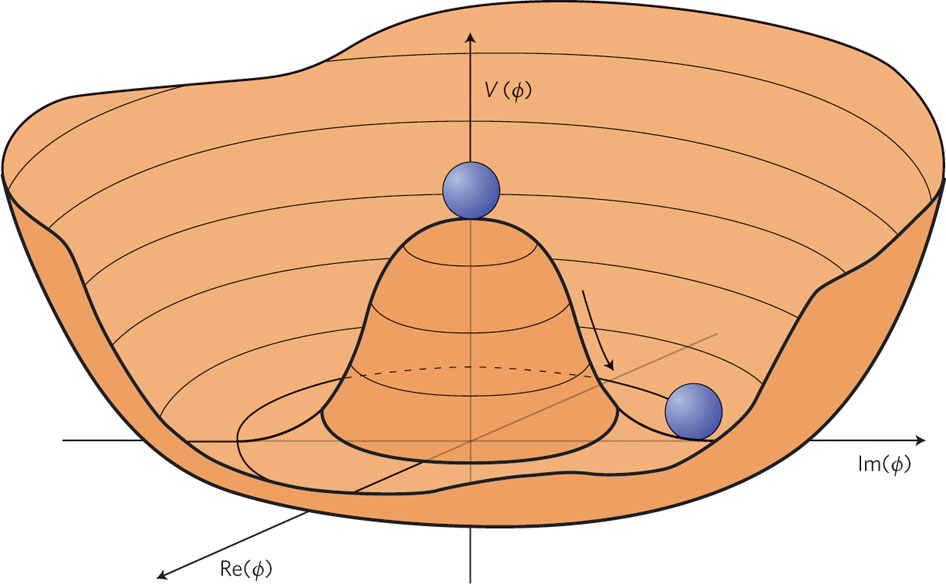
\includegraphics[width=.7\textwidth]{figures/Higgs-potential.jpg}
\caption{The non-zero vacuum potential of Higgs field. The $Im(\phi)$ and $Re(\phi)$ axes represent
the plane of space and time. The $V(\phi)$ axis represents the potential energy. And the circle
on top of the concave potential is the Higgs particle.}
\label{fig:Higgs}
\end{figure}  


The $W^+$, $W^-$ and Z bosons gain their masses through the spontaneous electroweak symmetry breaking mechanism.
In an unbroken unified electroweak theory, there are four types of massless bosons: W1, W2, W3, and X. And there are also four types of Higgs particles, which can not be distinguished from each other. After spontaneous symmetry breaking, these four Higgs particles become distinguishable: charged $H^+$, $H^-$, and neutral $H_0$ and $h$. 
The W1 boson coupling with the $H^+$ becomes the massive $W^+$ boson. The W2 coupling
with the $H^-$ becomes the $W^-$ boson. The W3 boson combined with the X boson together coupling with the $H_0$ becomes the Z boson. And the residual component of W3 and X combination becomes the massless photon. 

The $h$, as one of the four Higgs bosons, is not absorbed by other particles, which is called
the Higgs particle in SM.  However, there is no constraint on the mass of this Higgs particle in SM.



%The connection between symmetries and physics is deep. Noether's theorem states, essentially, that for every continuous symmetry of Nature there is a corresponding conservation law. 
%The construction of the Standard Model has been guided by principles of symmetry and also 
%symmetry breaking. 
\section{The physics beyond the SM}

Although the SM explains a lot of facts of current experiments and also achieves another tremendous success on 
the discovery of the SM-like Higgs boson in 2012. However, the SM cannot explain several
important phenomena, and thus it is believed to be an effective theory of a more fundamental
theory. 

{\bf Dark matter and dark energy}

%``More is unknown than is known" (quoted form NASA website). 
As shown in Figure~\ref{fig:universe}, the universe is expanding. However, the expansion is accelerating, instead of slowing down. 
Thus there must be some mysterious force overcomes the attractive force of gravity ad  
causes the accelerated expansion with time. 
This unknown force, is usually referred to as "dark energy". Dark here is 
the thing invisible to us. 

The need for dark matter arises from the astronomy observations that the rotational motion of 
the stars or galaxies suggests a $5{\sim}10$ times larger gravitational force than the one could be provided 
by the matter of the clusters. The lack of matter in this kind of case indicates the existence of 
matter that couldn't be observed by us, which is called ``dark matter".   
 
The current compositions of matter and energy of our universe, from studies, are about 4.9\% normal matter (like stars, planets, etc.), 26.8\% dark matter, and 68.3\% dark energy. The neutrinos of the SM, are stable and have tiny masses, and also interact weakly with other particles. So on a cosmic scale, they behave like 
the dark matter. However, the redundancy of dark matter (26.8\%) over normal matter (4.9\%) suggests that neutrinos are insufficient to explain the observed amount of dark matter. 

\begin{figure}[htbp]
\centering
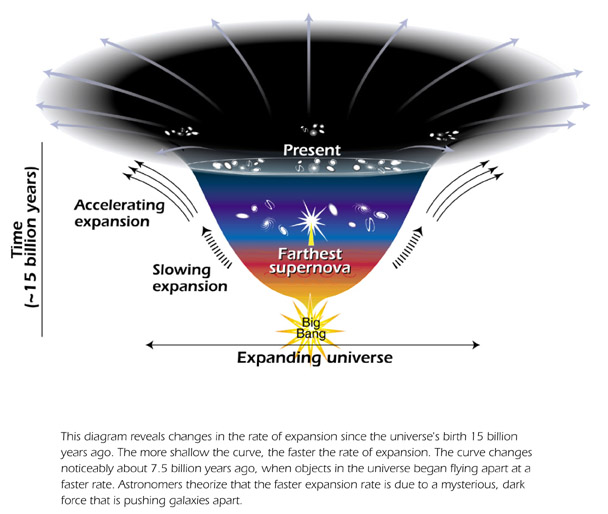
\includegraphics[width=.7\textwidth]{figures/accelerating_universe.jpg}
\caption{Accelerating expansion of the universe~\cite{web:nasa}.}
\label{fig:universe}
\end{figure}  



{\bf The hierarchy problem}

As shown in Table~\ref{table:fourForces}, the gravitational force is quite small compared 
to other three forces. It is about $10^{-30}$ smaller than the weak force. 
This large discrepancy of scale is called the 
hierarchy problem of the SM. 

The more formal way to state the hierarchy problem is why the Higgs mass in SM is in the scale of
${\approx}125$ GeV, 
rather not $10^{18}$ GeV, while the latter is more natural~\cite{wb:hierarchy}. 


\iffalse
{\color{red} Let's first introduce the higgs mechanism}
The hierarchy problem arises from the fact that as a scaler particle, with zero spin, the Higgs 
mass calculation using Feynman diagrams will eventually break down (divergent integral), which 
suggests Higgs particle possesses a large mass, about the Planck mass scale ($10^{18}$~GeV), which is the 
energy scale where our theory breaks down. 
However, in SM, Higgs boson accounts for the mass of W, Z, and all the fermions, through the 
mechanism of electroweak symmetry breaking. Although not confined, 
the SM H mass is preferably to be around $100$~GeV-ish, to account for 
the scattering process of longitudinally polarized vector bosons.  

%The recent discovered SM-like Higgs boson has a mass ${\approx} 125$~GeV, which 
\fi

{\bf Baryon-anitbaryon asymmetry }

The imbalance in baryonic matter and anti-baryonic matter in our observed universe
can not be explained by the SM, while the Big Bang should produce equal amount of 
matter and antimatter. 


{\bf Gravitation}

 The graviton is the mediator for gravitational force in SM. However, it has not been found yet. 
 Unlike the QED and QCD, there is no known way to explain relativity in SM. 
 \\
 
 
Since SM leaves us a lot of mysteries,  the scientific research towards a better understanding of 
 our universe has never been stopped. Several theories beyond the SM are raised. 
 Composite models of quarks (q*)~\cite{ref_qstar, ref_qstar2} with their potential to explain the generation structure of 
quarks have been quite popular. The Randall-Sundrum model with its potential to solve the
hierarchy problem in SM predicts the existence of 
Randall-Sundrum Graviton (\GRS)~\cite{rs1,Randall:1999vf}. 
There are also extensions of Randall-Sundrum models predicting the existence of 
bulk Graviton ($\GBulk$)~\cite{GravitonWWZZ1,GravitonWWZZ2,GravitonWWZZ3}. Many theories beyond the SM also predict the existence of 
\wpr and \zpr~\cite{egm}, the heavy partners of the SM W and Z bosons. 

According to experimental measurements, these predicted resonances are expected 
to have resonance masses at least a few hundred~GeV.  The Large Hadron Collider (LHC), 
with its high collision energy, is a great farm to possibly produce these massive resonances. 
%Most of these models of physics beyond the SM predict the
%existence of resonances with masses above 1~\TeVcc~ that decay into a
%quark and a \PW\ or \cPZ\ vector boson, or into two bosons (WW, ZZ, WZ, WH, or ZH).
The predicted massive resonances decaying into a quark and a \PW\ or \cPZ\ vector boson, or into two bosons (WW, ZZ, WZ, WH, or ZH) are searched in this thesis. 

In proton-proton (pp) collisions at the energies reached at the LHC, bosons emerging from such decays usually would have
sufficiently large momenta so that the hadronization products of their
$\qqbarprime$ decays would merge into a single massive
jet~\cite{Gouzevitch:2013qca}. So the event has a 
dijet topology.  
In this thesis, two dijet searches for physics beyond the SM are 
conducted with the CMS detector at LHC. 





